% ====================
\section{Introduction}
\label{mink_sec:intro}
% ====================

Given two sets $A,B \in \mathbb{R}^d$, their \emph{Minkowski sum},
denoted by $A \oplus B$, is the set $\left\{ a + b ~|~ a \in
A, b \in B \right\}$. Minkowski sum are used in many applications,
such as motion planning and computer-aided design and
manufacturing. This package contains functions for computing planar
Minkowski sums of two polygons (namely $A$ and $B$ are two closed
polygons in $\mathbb{R}^2$), and for a polygon and a disc (an operation
also known as \emph{offsetting} or \emph{dilating} a polygon).

\section{Computing the Minkowski Sum of Two Polygons}
\label{mink_sec:sum_poly}
%====================================================

Computing the Minkowski sum of two convex polygons $P$ and $Q$ with
$m$ and $n$ vertices respectively is very easy, as $P \oplus Q$ is a
convex polygon bounded by copies of the $m + n$ edges, and these edges
are sorted by the angle they form with the $x$-axis. As the two
input polygons are convex, their edges are already sorted by the
angle they form with the $x$-axis. The Minkowski sum can therefore be
computed in $O(m + n)$ time, by starting from two bottommost vertices
in $P$ and in $Q$ and performing ``merge sort'' on the edges.

\begin{figure}[t]
  \begin{ccTexOnly}
    \begin{center}
      \begin{tabular}{c c}
        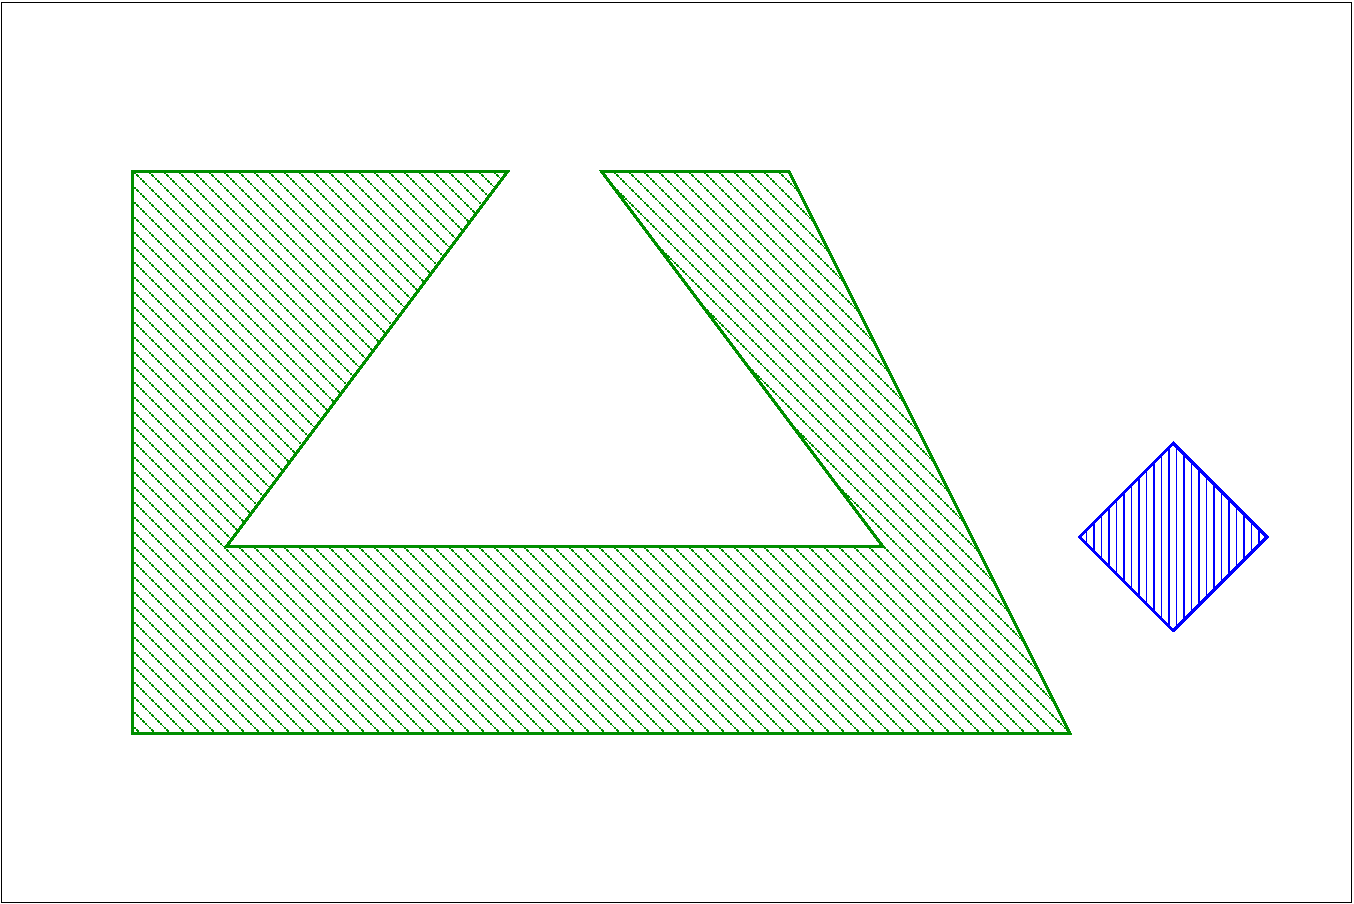
\includegraphics{Minkowski_sum_2/fig/onecyc_in} ~&~
        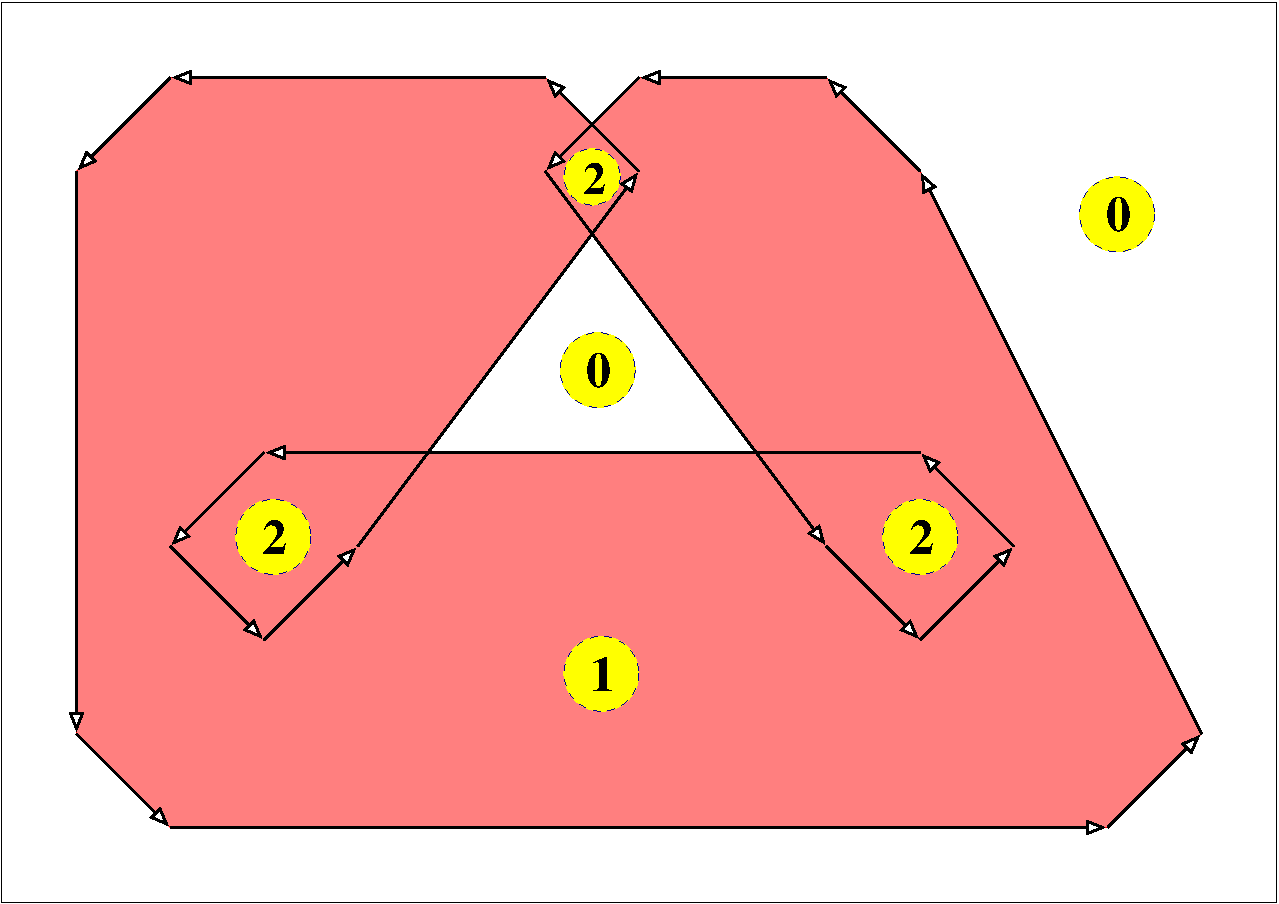
\includegraphics{Minkowski_sum_2/fig/onecyc_out}
      \end{tabular}
    \end{center}
  \end{ccTexOnly}
  \begin{ccHtmlOnly}
    <p><center>
    <table>
    <tr>
    <td><img src="./fig/onecyc_in.gif" border=0 alt="Convolution cycle"></td>
    <td><img src="./fig/onecyc_out.gif" border=0 alt="Convolution cycle"></td>
    </tr>
    </table>
    </center>
  \end{ccHtmlOnly}
\caption{Computing the convolution of a convex polygon and a
non-convex polygon (left). The convolution consists of a single
self-intersecting cycle, drawn as a sequence of arrows (right).
The winding number associated with each face of the arrangement
induced by the segments forming the cycle appears in dashed circles.
The Minkowski sum of the two polygons is shaded.}
\label{mink_fig:onecyc}
\end{figure}

If the polygons are not convex, it is possible to use one of the following
approaches:
\begin{description}
\item[Decomposition:]
We decompose $P$ and $Q$ into convex sub-polygons, namely we obtain two
sets of convex polygons $P_1, \ldots, P_k$ and $Q_1, \ldots, Q_\ell$ such
that $\bigcup_{i = 1}{k}{P_i} = P$ and $\bigcup_{i = j}{\ell}{Q_j} = Q$.
We then calculate the pairwise sums $S_{ij} = P_i \oplus Q_j$ using the
simple procedure described above, and compute the union $P \oplus Q =
\bigcup_{ij}{S_{ij}}$.

This approach relies on a decomposition strategy that computes the convex
decomposition of the input polygons and its performance depends on the
quality of the decomposition.
%
\item[Convolution:]
Let us denote the vertices of the input polygons by
$P = \left( p_0, \ldots, p_{m-1} \right)$ and
$Q = \left( q_0, \ldots, q_{n-1} \right)$. We assume that both $P$ and $Q$
have positive orientations (i.e. their boundaries wind in a counterclockwise
order around their interiors) and compute the convolution of the two polygon
boundaries. The {\em convolution} of these two polygons~\cite{grs-kfcg-83},
denoted $P * Q$, is a collection of line segments of the form
$[p_i + q_j, p_{i+1} + q_j]$,\footnote{Throughout this chapter, we increment
or decrement an index of a vertex modulo the size of the polygon.}
where the vector ${\mathbf p_i p_{i+1}}$
lies between ${\mathbf q_{j-1} q_j}$ and ${\mathbf q_j
q_{j+1}}$,\footnote{We say that a vector ${\mathbf v}$ lies between
two vectors ${\mathbf u}$ and ${\mathbf w}$ if we reach ${\mathbf v}$ strictly
before reaching ${\mathbf w}$ if we move all three vectors to the origin
and rotate ${\mathbf u}$ counterclockwise. Note that this also covers
the case where ${\mathbf u}$ has the same direction as ${\mathbf v}$.} and
--- symmetrically --- of segments of the form $[p_i + q_j, p_i + q_{j+1}]$,
where the vector ${\mathbf q_j q_{j+1}}$ lies between
${\mathbf p_{i-1} p_i}$ and ${\mathbf p_i p_{i+1}}$.

The segments of the convolution form a number of closed (not
necessarily simple) polygonal curves called \emph{convolution
cycles}. The Minkowski sum $P \oplus Q$ is the set of points
having a non-zero winding number with respect to the cycles
of $P * Q$.\footnote{Informally speaking, the winding number of a point
$p \in \mathbb{R}^2$ with respect to some planar curve $\gamma$ is an
integer number counting how many times does $\gamma$ wind in a
counterclockwise direction around $p$.} See Figure~\ref{mink_fig:onecyc}
for an illustration.

The number of segments in the convolution of two polygons is usually
smaller than the number of segments that constitute the boundaries of the
sub-sums $S_{ij}$ when using the decomposition approach. As both approaches
construct the arrangement of these segments and extract the sum from this
arrangement, computing Minkowski sum using the convolution approach usually
generates a smaller intermediate arrangement, hence it is faster and
consumes less space.
\end{description}

\subsection{Computing Minkowski Sum using Convolutions}
\label{mink_ssec:sum_conv}
%------------------------------------------------------

The function \ccc{minkowski_sum_2 (P, Q)} accepts two simple polygons $P$
and $Q$, represented using the \ccc{Polygon_2<Kernel,Container>}
class-template and uses the convolution method in order to compute and
return their Minkowski sum $S = P \oplus Q$.

As the input polygons may not be convex,their Minkowski sum may not be
simply connected and contain polygonal holes; see for example
Figure~\ref{mink_fig:onecyc}. $S$ is therefore an instance of the
\ccc{Polygon_with_holes_2<Kernel,Container>} class-template, defined in the
Boolean Set-Operations package: The outer boundary of $S$ is a polygon that
can be accessed using \ccc{S.outer_boundary()}, and its polygonal holes can
are given by the range \ccc{[S.holes_begin(), S.holes_end())} (where $S$
contains \ccc{S.number_of_holes()} holes in its interior).

\begin{figure}[t]
\begin{ccTexOnly}
  \begin{center}
    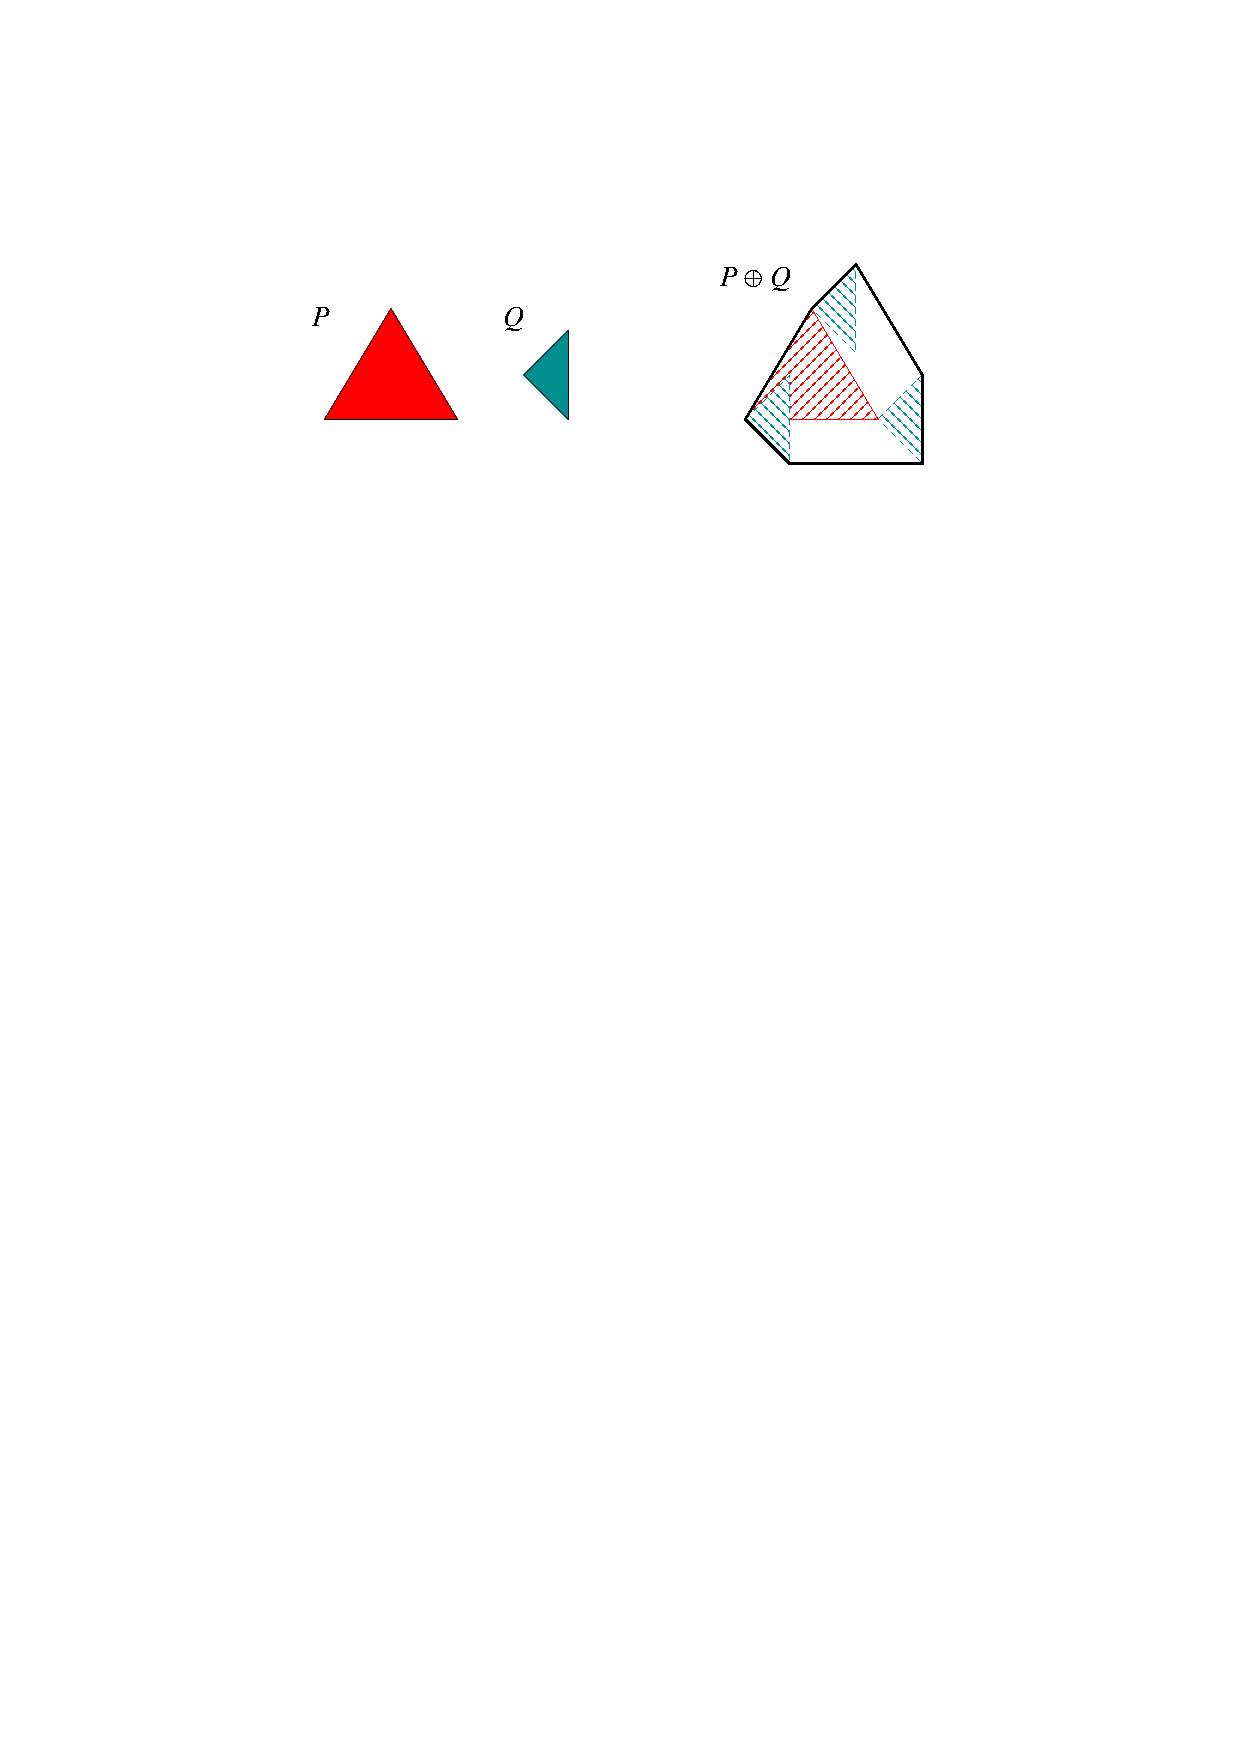
\includegraphics{Minkowski_sum_2/fig/sum_triangles}
  \end{center}
\end{ccTexOnly}
\begin{ccHtmlOnly}
  <p><center>
  <img src="./fig/sum_triangles.gif" border=0 alt="Minkowski sum of two triangles">
  </center>
\end{ccHtmlOnly}
\caption{Computing the Minkowski sum of two triangles, as done
in the example program \ccc{ex_sum_triangles.cpp}.}
\label{mink_fig:sum_tri}
\end{figure}

The following example program constructs the Minkowski sum of two triangles,
as depicted in Figure~\ref{mink_fig:sum_tri}. The result in this case is
a convex hexagon. This program, as other example programs in this chapter,
includes the auxiliary header file \ccc{ms_rational_nt.h} which defines
\ccc{Number_type} as either \ccc{Gmpq} or \ccc{Quotient<MP_Float>},
depending on whether the {\sc Gmp} library is installed or not.
The file \ccc{print_util.h} includes auxiliary functions for printing polygons.

\ccIncludeExampleCode{../examples/Minkowski_sum_2/ex_sum_triangles.cpp}

\begin{figure}[t]
\begin{ccTexOnly}
  \begin{center}
    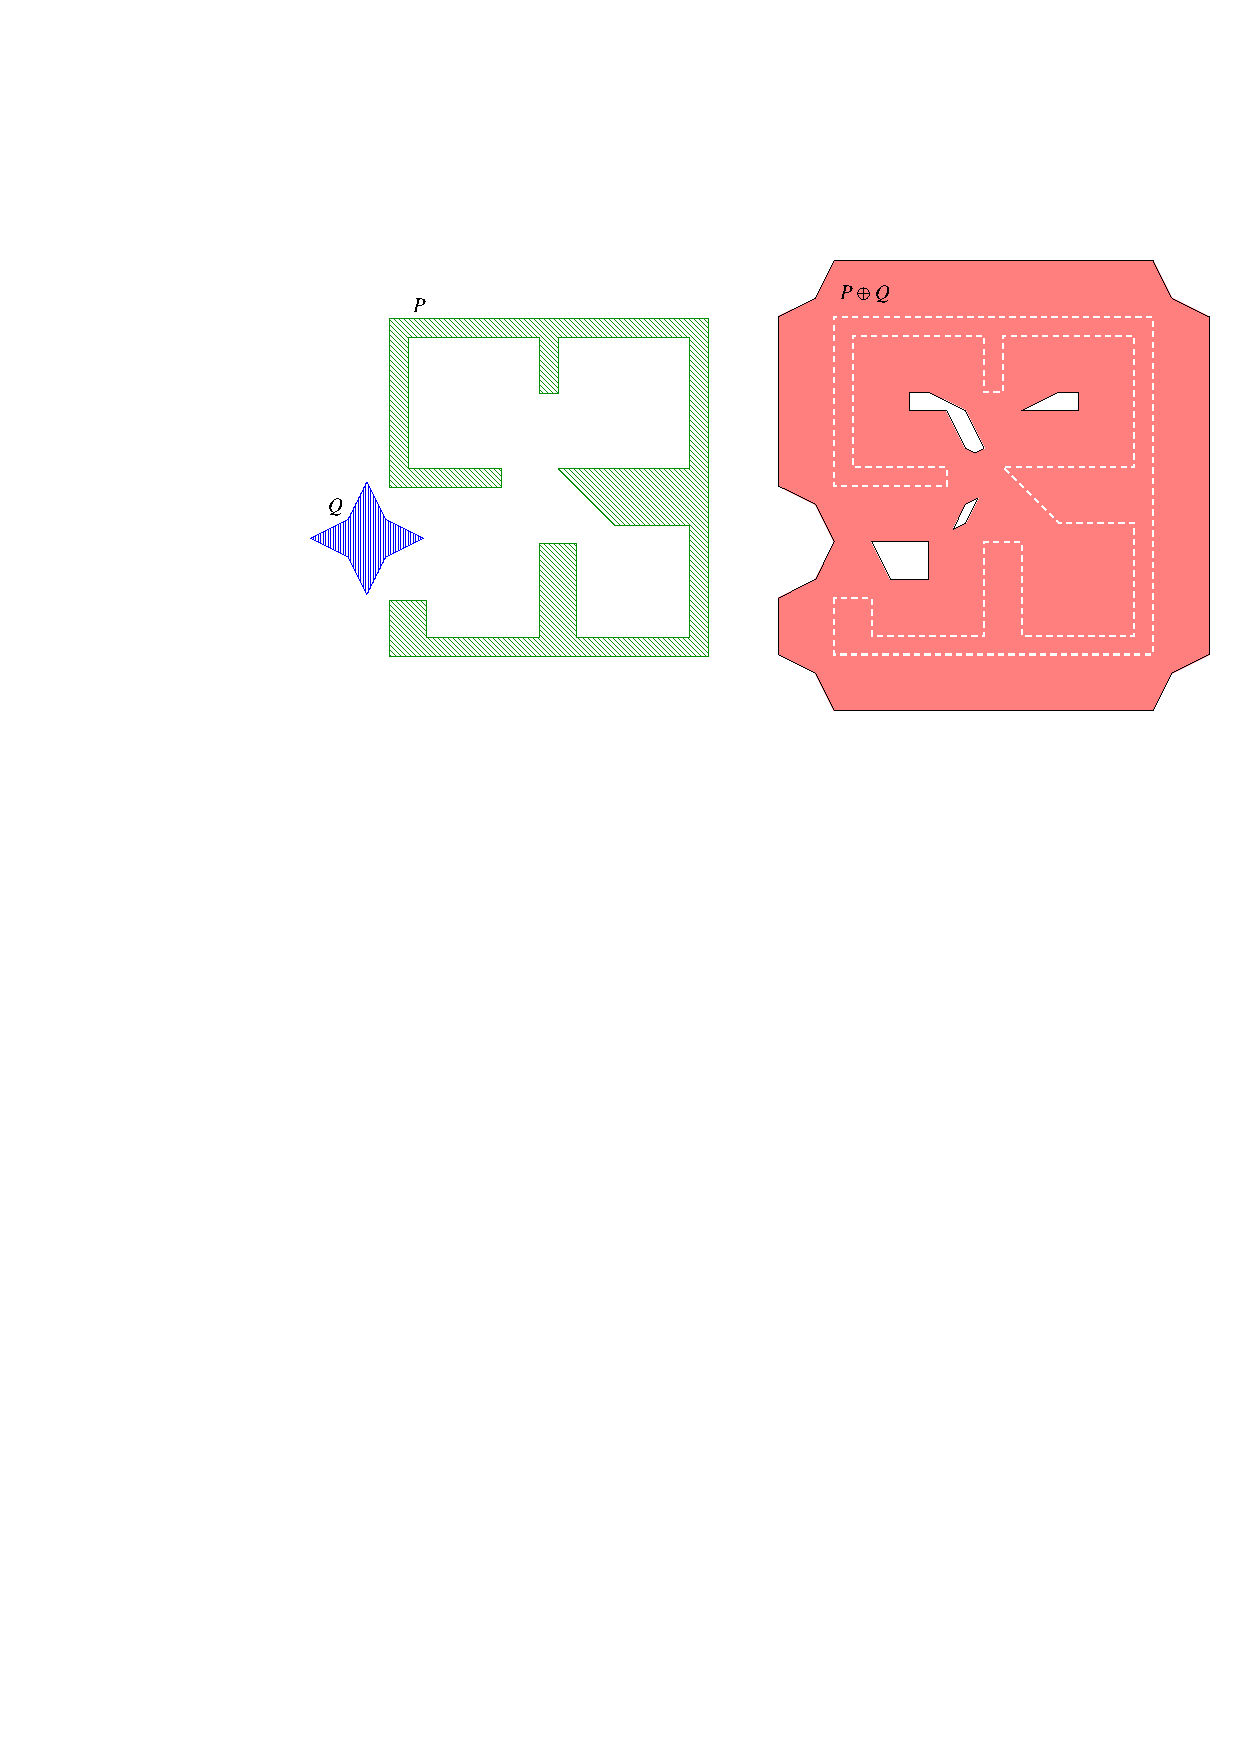
\includegraphics{Minkowski_sum_2/fig/tight}
  \end{center}
\end{ccTexOnly}
\begin{ccHtmlOnly}
  <p><center>
  <img src="./fig/tight.gif" border=0 alt="Minkowski sum of two non-convex polygon that contains holes">
  </center>
\end{ccHtmlOnly}
\caption{Computing the Minkowski sum of two non-convex polygons $P$ and $Q$,
as done in the example programs \ccc{ex_sum_with_holes.cpp} and
\ccc{ex_sum_by_decomposition.cpp}.}
\label{mink_fig:sum_holes}
\end{figure}

In the following program we compute the Minkowski sum of two polygons
that are read from an input file. In this case, the sum is not simple
and contains four holes, as illustrated in Figure~\ref{mink_fig:sum_holes}.
Note that this example uses the predefined \cgal\ kernel with exact
constructions. In general, instantiating polygons with this kernel yields
the fastest running times for Minkowski-sum computations.

\ccIncludeExampleCode{../examples/Minkowski_sum_2/ex_sum_with_holes.cpp}

\subsection{Decomposition Strategies}
\label{mink_ssec:decomp}
%------------------------------------

In order to compute Minkowski sums using the decomposition method, it is
possible to call the function \ccc{minkowski_sum_2 (P, Q, decomp)}, where
\ccc{decomp} is an instance of a class that models the concept
\ccc{PolygonConvexDecomposition_2}, namely it should provide a method named
\ccc{decompose()} that receives a planar polygons and returns a range
of convex polygons that represents its convex decomposition.

The Minkowski-sum package includes four models of the concept
\ccc{PolygonConvexDecomposition_2}. The first three are classes that wrap
the decomposition functions included in the Planar Polygon Partitioning
package, while the fourth is an implementation of a decomposition algorithm
introduced in~\cite{cgal:afh-pdecm-02}. The convex decompositions that it
creates usually yield efficient running times for Minkowski sum computations:
\begin{itemize}
\item
The class \ccc{Optimal_convex_decomposition<Kernel>} uses the
dynamic-programming algorithm of Greene~\cite{g-dpcp-83} for computing an
optimal decomposition of a polygon into a minimal number of convex
sub-polygons. The main drawback of this strategy is that it runs in $O(n^4)$
time and $O(n^3)$ in the worst case,where $n$ is the number of vertices in
the input polygon.
%
\item
The class \ccc{Hertel_Mehlhorn_convex_decomposition<Kernel>} implements the
approximation algorithm suggested by Hertel and Mehlhorn~\cite{hm-ftsp-83},
which triangulates the input polygon and proceeds by throwing away
unnecessary triangulation edges.
This algorithm requires $O(n)$ time and space and guarantees that
the number of sub-polygons it generates is not more than four
times the optimum.
%
\item
The class \ccc{Greene_convex_decomposition<Kernel>} is an implementation of
Greene's approximation algorithm~\cite{g-dpcp-83}, which computes a
convex decomposition of the polygon based on its partitioning into
$y$-monotone polygons. This algorithm runs in $O(n \log n)$ time
and $O(n)$ space, and has the same approximation guarantee as
Hertel and Mehlhorn's algorithm.
%
\item
The class \ccc{Small_side_angle_bisector_convex_decomposition<Kernel>} uses
a heuristic improvement to the angle-bisector decomposition method
suggested by Chazelle and Dobkin~\cite{cd-ocd-85}, which runs in
$O(n^2)$ time. It starts by examining each pair of reflex vertices
in the input polygon such that the entire interior of the diagonal
connecting these vertices is contained in the polygon. Out of all
available pairs, the vertices $p_i$ and $p_j$ are selected such
that the number of reflex vertices from $p_i$ to $p_j$ (or from
$p_j$ to $p_i$) is minimal. The polygon is split by the diagonal
$p_i p_j$ and we continue recursively on both resulting
sub-polygons. In case it is not possible to eliminate two reflex
vertices at once any more, each reflex vertex is eliminated by a
diagonal that is closest to the angle bisector emanating from this
vertex.
\end{itemize}

The following example demonstrates the computation of the Minkowski sum
of the same input polygons as used in \ccc{ex_sum_with_holes.cpp} (as
depicted in Figure~\ref{mink_fig:sum_holes}), using the small-side
angle-bisector decomposition strategy:

\ccIncludeExampleCode{../examples/Minkowski_sum_2/ex_sum_by_decomposition.cpp}

\section{Offsetting a Polygon}
\label{mink_sec:offset}
%=============================

The operation of computing the Minkowski sum $P \oplus B_r$ of a
polygon $P$ with $b_r$, a disc of radius $r$ centered at the origin,
is widely known as \emph{offsetting} the polygon $P$ by a radius $r$.

\begin{figure}[t]
\begin{ccTexOnly}
\begin{center}
  \begin{tabular}{ccc}
    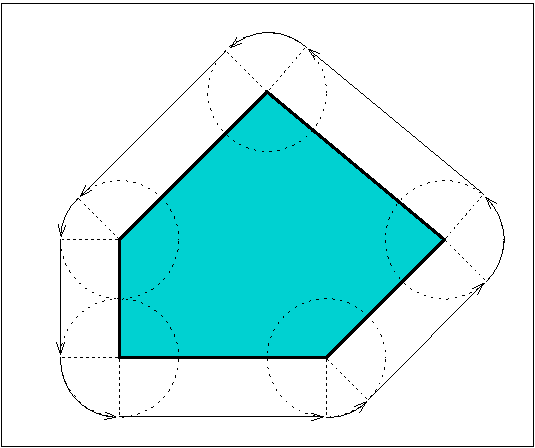
\includegraphics{Minkowski_sum_2/fig/convex_offset} &
    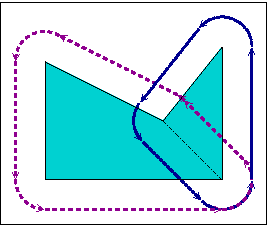
\includegraphics{Minkowski_sum_2/fig/offset_decomp} &
    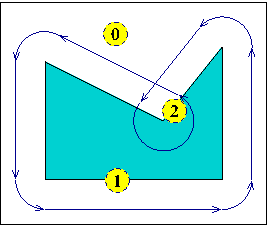
\includegraphics{Minkowski_sum_2/fig/offset_conv} \\
    {\small (a)} & {\small (b)} & {\small (c)}
  \end{tabular}
\end{center}
\end{ccTexOnly}
\begin{ccHtmlOnly}
  <p><center>
  <table>
  <tr>
  <td><img src="./fig/convex_offset.gif" border=0 alt="Computing offsets of polygons"></td>
  <td><img src="./fig/offset_decomp.gif" border=0 alt="Computing offsets of polygons"></td>
  <td><img src="./fig/offset_conv.gif" border=0 alt="Computing offsets of polygons"></td>
  </tr>
  <tr align="center"><td>(a)</td><td>(b)</td><td>(c)</td></tr>
  </table>
  </center>
\end{ccHtmlOnly}
\caption{(a)~Offsetting a convex polygon.
(b)~Computing the offset of a non-convex polygon by decomposing
it to convex sub-polygons. (c)~Offsetting a non-convex polygon
by computing its convolution with a disc. The convolution cycle
induces an arrangement with three faces, whose winding numbers
are shown enclosed in dashed circles.}
\label{mink_fig:pgn_offset}
\end{figure}

Let $P = \left( p_0, \ldots, p_{n - 1} \right)$ be the polygon vertices,
ordered in a counterclockwise orientation around its interior. 
If $P$ is a convex polygon the offset is easily computed by
shifting each polygon edge by $r$ away from the polygon, namely to
the right side of the edge. As a result we obtain a collection of
$n$ disconnected \emph{offset edges}. Each pair of adjacent offset
edges, induced by $p_{i-1} p_i$ and $p_i p_{i+1}$, are connected
by a circular arc of radius $r$, whose supporting circle is
centered at $p_i$. The angle that defines such a circular arc
equals $180^{\circ} - \angle (p_{i-1}, p_i, p_{i+1})$; see
Figure~\ref{mink_fig:pgn_offset}(a) for an illustration. The running
time of this simple process is of course linear with respect to
the size of the polygon.

If $P$ is not convex, its offset can be obtained by decomposing it
to convex sub-polygons $P_1, \ldots P_m$ such that
$\bigcup_{i=1}^{m}{P_i} = P$, computing the offset of each
sub-polygon and finally calculating the union of these sub-offsets
(see Figure~\ref{fig:pgn_offset}(b)). However, as was the case with
the Minkowski sum of a pair of polygons, here it is also more
efficient to compute the \emph{convolution cycle} of the polygon
with the disc $B_r$,\footnote{As the disc is convex, it is guaranteed
that the convolution curve is comprised of a single cycle.} which can be
constructed by applying the process described in the previous
paragraph. The only difference is that a circular arc induced by a
reflex vertex $p_i$ is defined by an angle $540^{\circ} - \angle
(p_{i-1}, p_i, p_{i+1})$; see Figure~\ref{fig:pgn_offset}(c) for an
illustration. We finally compute the winding numbers of the faces of the
arrangement induced by the convolution cycle to obtain the offset
polygon.

\subsection{Approximating the Offset with a Guaranteed Error-Bound}
\label{mink_ssec:approx_offset}
%------------------------------------------------------------------

Let us assume that we are given a counterclockwise-oriented polygon
$P = \left( p_0, \ldots, p_{n-1} \right)$, whose vertices all have rational
coordinates (i.e., for each vertex $p_i = (x_i, y_i)$ we have
$x_i, y_i \in {\mathbb Q}$, and we wish to compute its Minkowski sum with a
disc of radius $r$, where $r$ is also a rational number. The boundary of this
sum is comprised of line segments an circular arcs, where:
\begin{itemize}
\item
Each circular arc is supported by a circle of radius $r$ centered at one
of the polygon vertices. The equation of this circle is $(x - x_i)^2 +
(y - y_i)^2 = r^2$, and has only rational coefficients.
%
\item
Each line segment is supported by a line parallel to one of the polygon
edges $p_i p_{i+1}$, which lies at distance $r$ from this edge. If we 
denote the supporting line of $p_i p_{i+1}$ by $ax + by + c = 0$, where
$a, b, c \in {\mathbb Q}$, then the offset edge is supported by the line
$ax + by + (c + \ell\cdot r) = 0$, where $\ell$ is the length of the edge
$p_i p_{i+1}$ and is in general \emph{not} a rational number. The line segments
that comprise the offset boundaries therefore cannot be represented as segments
of lines with rational coefficients.
%
We mention that the locus of all points that lie at distance $r$ from the
line $ax + by + c = 0$ is given by:
\[ \frac{(ax + by + c)^2}{a^2 + b^2} = r^2 \ .\]
Thus, the linear offset edges are segments of curves of an algebraic curve
of degree 2 (a conic curve) with rational coefficients. This curve is
actually a pair of the parallel lines $ax + by + (c \pm \ell\cdot r) = 0$.
In Section~\ref{mink_ssec:exact_offset} we use this representation to
construct the offset polygon in an exact manner using the traits class for
conic arcs.
\end{itemize}

\begin{figure}[t]
\begin{ccTexOnly}
  \begin{center}
  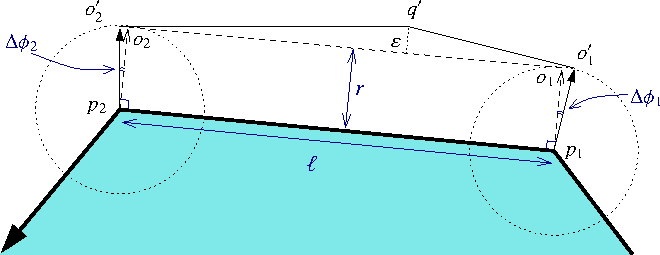
\includegraphics{Minkowski_sum_2/fig/approx_offset}
  \end{center}
\end{ccTexOnly}
\begin{ccHtmlOnly}
  <p><center>
  <img src="./fig/approx_offset.gif" border=0 alt="Approximating an offset edge">
  </center>
\end{ccHtmlOnly}
\caption{Approximating the offset edge $o_1 o_2$ induced by the polygon
edge $p_1 p_2$ by two line segments $o'_1 q'$ and $q' o'_2$.}
\label{mink_fig:approx_offset}
\end{figure}

The class-template \ccc{Gps_circle_segment_traits_2<Kernel>}, included in
the Boolean Set-Operations package is used for representing general polygons
whose edges are circular arcs or line segments, and for applying set operations
(e.g. intersection, union, etc.) on such general polygon. It should be
instantiated with a geometric kernel that employs exact rational arithmetic,
such that the curves that comprise the polygon edges should be arcs of
circles with rational coefficients or segments of lines with rational
coefficients. As in our case the line segments do not satisfy this requirement,
we apply a simple approximation scheme, such that each irrational line
segment is approximated by two rational segments:
\begin{enumerate}
\item
Consider the example depicted in Figure~\ref{mink_fig:approx_offset}, where
the exact offset edge $o_1 o_2$ is obtained by shifting the polygon edge
$p_1 p_2$ by a vector whose length is $r$ that form an angle $\phi$ with the
$x$-axis. We select two points $o'_1$ and $o'_2$ with rational coordinates
on the two circles centered at $p_1$ and $p_2$, respectively. These points
are selected such that if we denote the angle that the vector 
${\mathbf p_j o_j}$
forms with the $x$-axis by $\phi'_j$ (for $j = 1, 2$), we have
$\phi'_1 < \phi < \phi'_2$.
%
\item
We construct two tangents to the two circles at $o'_1$ and $o'_2$,
respectively. The tangent lines have rational coefficients.
%
\item
We compute the intersection point of the two tangents, denoted $q'$.
The two line segments $o'_1 q'$ and $q' o'_2$ approximate the original
offset edge $o_1 o_2$.
\end{enumerate}

The function \ccc{approximated_offset_2 (P, r, eps)} accepts a polygon
$P$, an offset radius $r$ and $\varepsilon > 0$. It constructs an
approximation for the offset of $P$ by the radius $r$ using the procedure
explained above. Furthermore, it is guaranteed that the approximation error,
namely the distance of the point $q'$ from $o_1 o_2$ is bounded by
$\varepsilon$. Using this function, we are capable of working with the
\ccc{Gps_circle_segment_traits_2<Kernel>} class, which considerably
speeds up the (approximate) construction of the offset polygon and the
application of set operations on such polygons. The function returns an
object of the nested type
\ccc{Gps_circle_segment_traits_2<Kernel>::Polygon_with_holes_2} representing
the approximated offset polygon (recall that if $P$ is not convex, its
offset may not be simple an contain holes, whose boundary is also comprised
of line segments and circular arcs).

\begin{figure}[t]
\begin{ccTexOnly}
  \begin{center}
    
\includegraphics{Minkowski_sum_2/fig/ex_offset} 
  \end{center}
\end{ccTexOnly}
\begin{ccHtmlOnly}
  <p><center>
  <img src="./fig/ex_offset.gif" border=0 alt="Offsetting a polygon">
  </center>
\end{ccHtmlOnly}
\caption{The offset computation performed by the example programs
\ccc{ex_approx_offset.cpp} and \ccc{ex_exact_offset.cpp}. The input polygon
is shaded and the boundary of its offset is drawn in a thick black line.}
\label{mink_fig:ex_offset}
\end{figure}

The following example demonstrates the construction of an approximated
offset of a non-convex polygon, as depicted in
Figure~\ref{mink_fig:ex_offset}. Note that we use a geometric kernel
parameterized with a filtered rational number-type. Using filtering
considerably speeds up the construction of the offset.

\ccIncludeExampleCode{../examples/Minkowski_sum_2/ex_approx_offset.cpp}

\subsection{Computing the Exact Offset}
\label{mink_ssec:exact_offset}
%--------------------------------------

As we previously mentioned, it is possible to represent offset polygons
in an exact manner, if we treat their edges as arcs of conic curves with
rational coefficients. The function \ccc{offset_polygon_2 (traits, P, r)}
computes the offset of the polygon $P$ by a rational radius $r$ in an
exact manner. The \ccc{traits} parameter should be an instance of an
arrangement-traits class that is capable of handling conic arcs in an
exact manner; using the \ccc{Arr_conic_traits_2} class with the number
types provided by the {\sc Core} library is the preferred option.
The function returns an object of the nested type
\ccc{Gps_traits_2<ArrConicTraits>::Polygons_with_holes_2} (see the
documentation of the Boolean Set-Operations package for more details
on the traits-class adapter \ccc{Gps_traits_2}), which represented the
exact offset polygon.

The following example demonstrates the construction of the offset
of the same polygon that serves as an input for the example program
\ccc{ex_approx_offset.cpp}, presented in the previous subsection (see also
Figure~\ref{mink_fig:ex_offset}). Note that the resulting polygon is
smaller than the one generated by the approximated-offset function (recall
that each irrational line segment in this case is approximated by two
rational line segments), but the offset computation is considerably slower:

\ccIncludeExampleCode{../examples/Minkowski_sum_2/ex_exact_offset.cpp}

\begin{ccAdvanced}
Both functions \ccc{approximated_offset_2()} and \ccc{offset_polygon_2()}
also have an overloaded versions that accept a decomposition strategy
and use the polygon-decomposition approach to compute (or approximate)
the offset. These functions are less efficient than their counterparts
that employ the convolution approach, and are only included in the package
for the sake of completeness.
\end{ccAdvanced}


